% Figure 18 - Region of two dimensions
% Independently revalidated against IEEE Std 1516.1-2010 source physical p.205.
% Natural source raster: 784 x 498, placed anisotropically at
% (116.8405,75.4163)..(491.7395,305.7828) PDF pt.
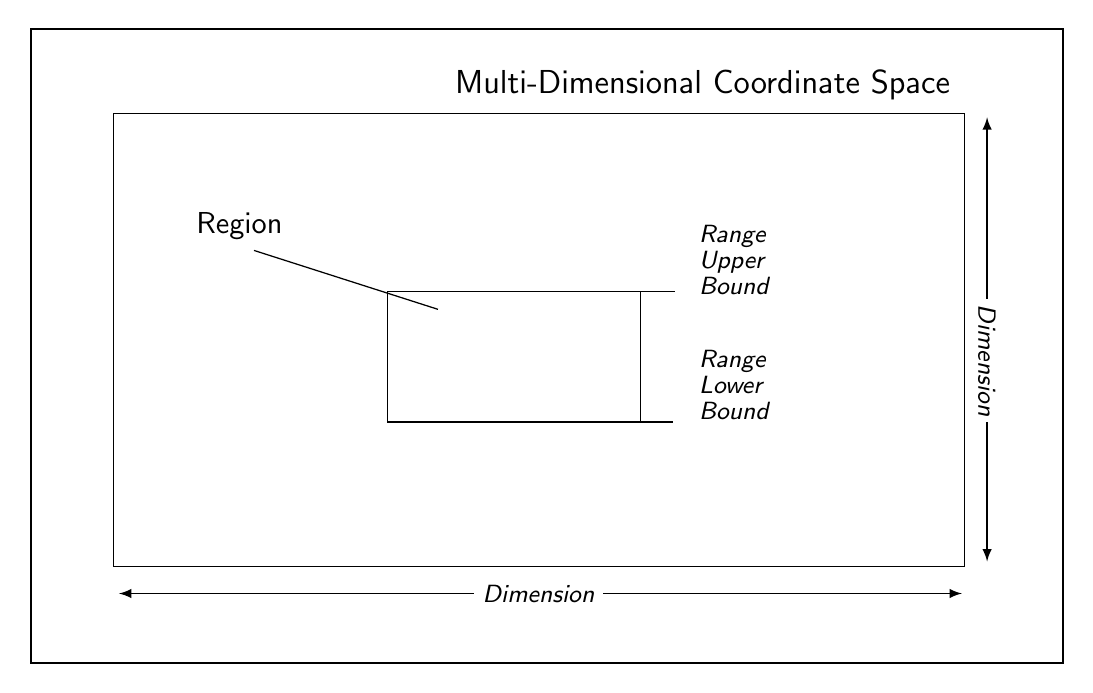
\begin{tikzpicture}[x=.4781875221pt,y=-.4625833350pt,line cap=butt,line join=miter,>=latex]
    \path[use as bounding box] (0,0) rectangle (784,498);

    % Source PDF draws this outside the one-bit figure image; included natively here.
    \draw[line width=.72pt] (2.22,1.05) rectangle (782.16,496.53);

    % Multi-dimensional coordinate-space box.
    \draw[line width=.45pt] (65,67) rectangle (708,421);
    \node[anchor=center,font=\sffamily\fontsize{11.5}{12.2}\selectfont] at (510,45)
        {Multi-Dimensional Coordinate Space};

    % Region realization.
    \draw[line width=.45pt] (272,206) rectangle (463,308);
    \draw[line width=.45pt] (463,206) -- (489,206);
    \draw[line width=.45pt] (463,308) -- (488,308);
    \node[anchor=center,font=\sffamily\fontsize{10.7}{11.4}\selectfont] at (160,155) {Region};
    \draw[line width=.45pt] (171,174) -- (310,220);

    % Range-bound labels.
    \node[anchor=west,align=left,font=\sffamily\itshape\fontsize{9.0}{9.4}\selectfont]
    at (500,181) {Range\\Upper\\Bound};
    \node[anchor=west,align=left,font=\sffamily\itshape\fontsize{9.0}{9.4}\selectfont]
    at (500,279) {Range\\Lower\\Bound};

    % Horizontal dimension indicator. The source line is interrupted by its label.
    \draw[line width=.55pt,<->] (69,442) -- (706,442);
    \node[fill=white,inner xsep=3.2pt,inner ysep=.2pt,
        font=\sffamily\itshape\fontsize{9.2}{9.6}\selectfont] at (386,442) {Dimension};

    % Vertical dimension indicator. The label masks the middle of the arrow line.
    \draw[line width=.55pt,<->] (725,70) -- (725,417);
    \node[fill=white,inner xsep=2.2pt,inner ysep=.3pt,rotate=-90,
        font=\sffamily\itshape\fontsize{9.2}{9.6}\selectfont] at (725,260) {Dimension};
\end{tikzpicture}
